\section*{\Huge{List of Annexes}}
\addcontentsline{toc}{chapter}{List of Annexes}

\subsection*{Annex 1 - Global History of Orange}
\begin{center}
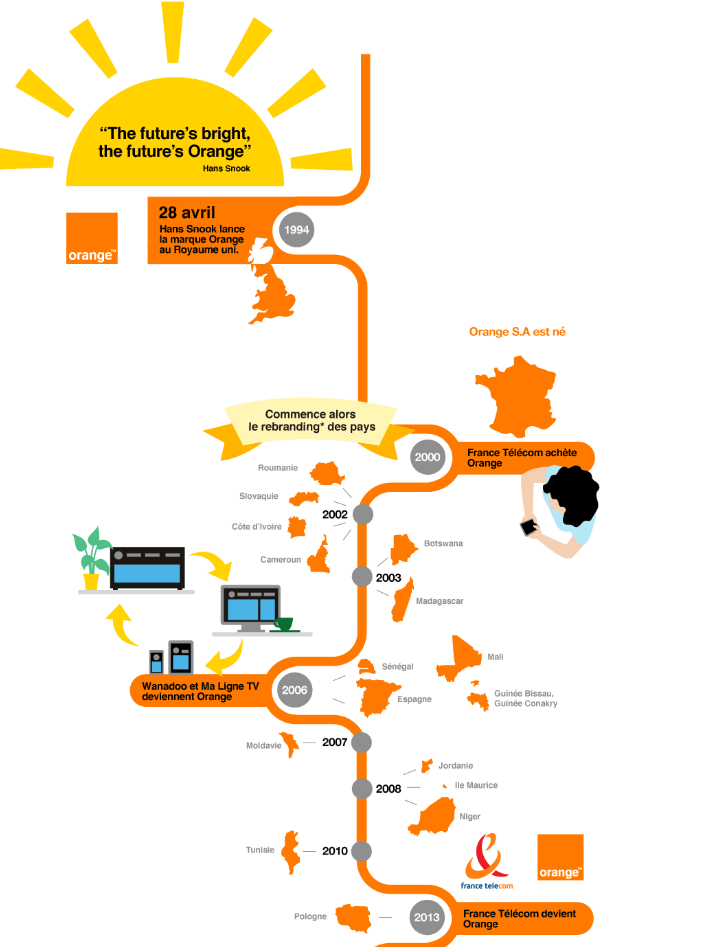
\includegraphics[scale=1.37]{annexs/Orange Histoire .PNG}
\end{center}

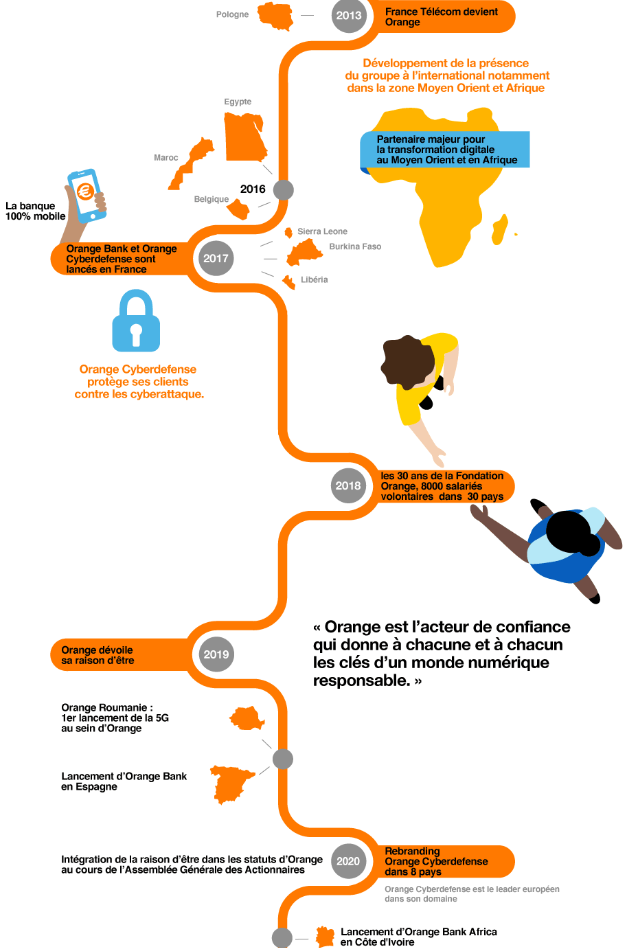
\includegraphics[scale=0.9]{annexs/Capture1.PNG}

\subsection*{Annex 2 - DRI Organization Chart}
\begin{center}
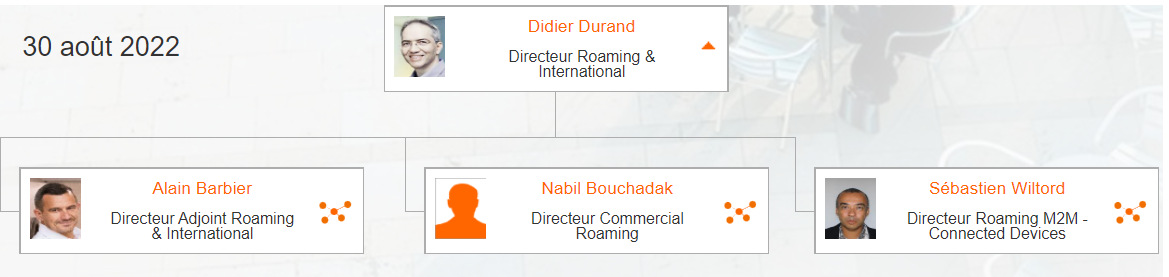
\includegraphics[scale=0.71]{annexs/Direction roaming et international.PNG}
\includegraphics[scale=0.71]{annexs/Alain barbier équipe.PNG}
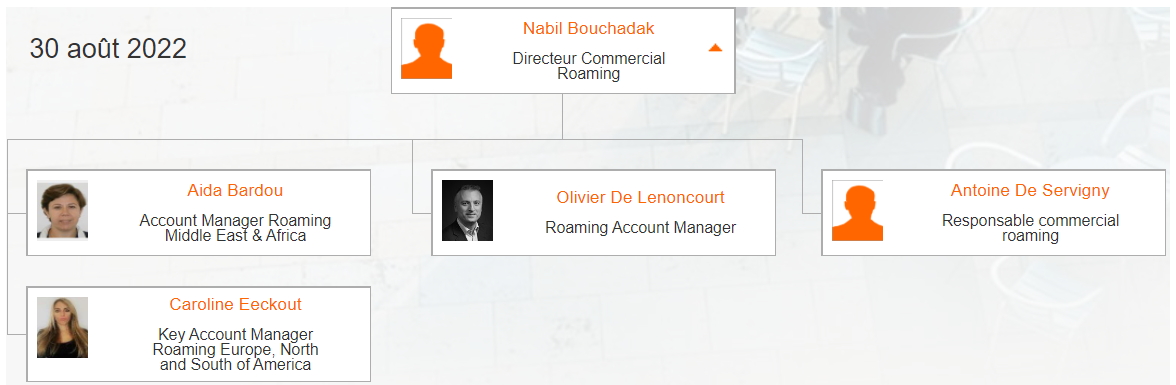
\includegraphics[scale=0.71]{annexs/commerciale team .PNG}
\includegraphics[scale=0.71]{annexs/Sébastien team.PNG}
\end{center}

\subsection*{Annex 3 - Roaming Definition}
\begin{center}
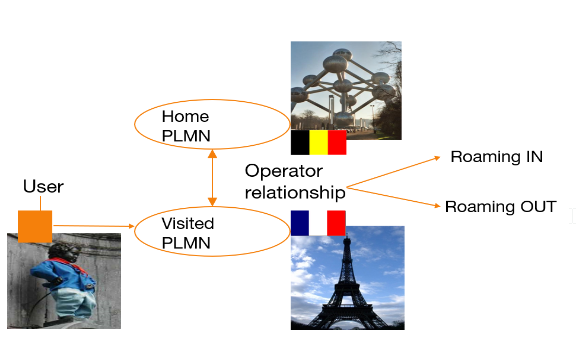
\includegraphics[scale=0.71]{annexs/romdef.PNG}
\end{center}

\subsection*{Annex 4 - Information exchange between roaming partners}
\begin{center}
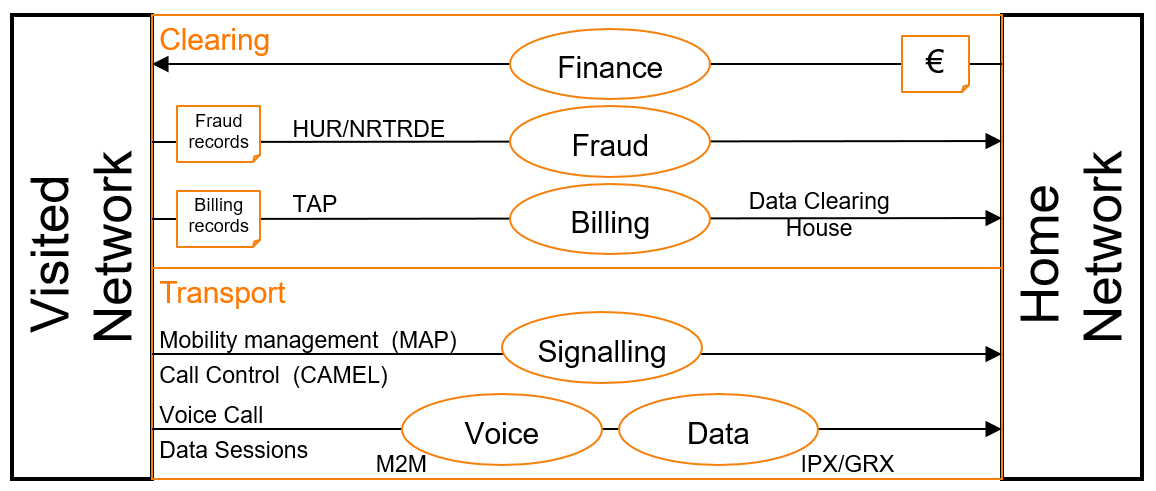
\includegraphics[scale=0.71]{annexs/Roaming relation .PNG}
\end{center}

\subsection*{Annex 5 - Overal Roaming Sponsor Architectur}
\begin{center}
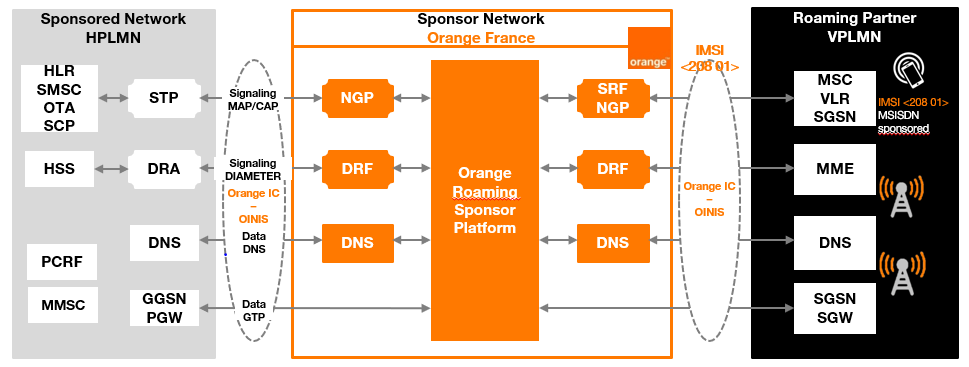
\includegraphics[scale=0.8]{annexs/Raoming sponsor architecture.PNG}
\end{center}

\subsection*{Annex 6 - Information exchange through roaming HUB}
\begin{center}
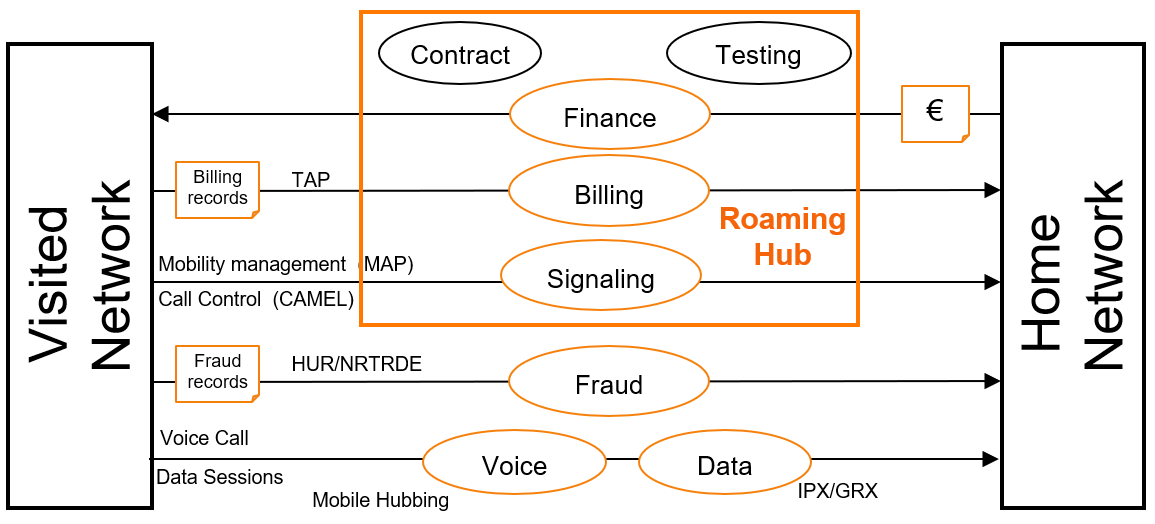
\includegraphics[scale=0.71]{annexs/roaming relation via hub.PNG}
\end{center}

\subsection*{Annex 7 - Presentation of olivera}
\subsubsection*{Home page - Ecran d’accueil}
\begin{center}
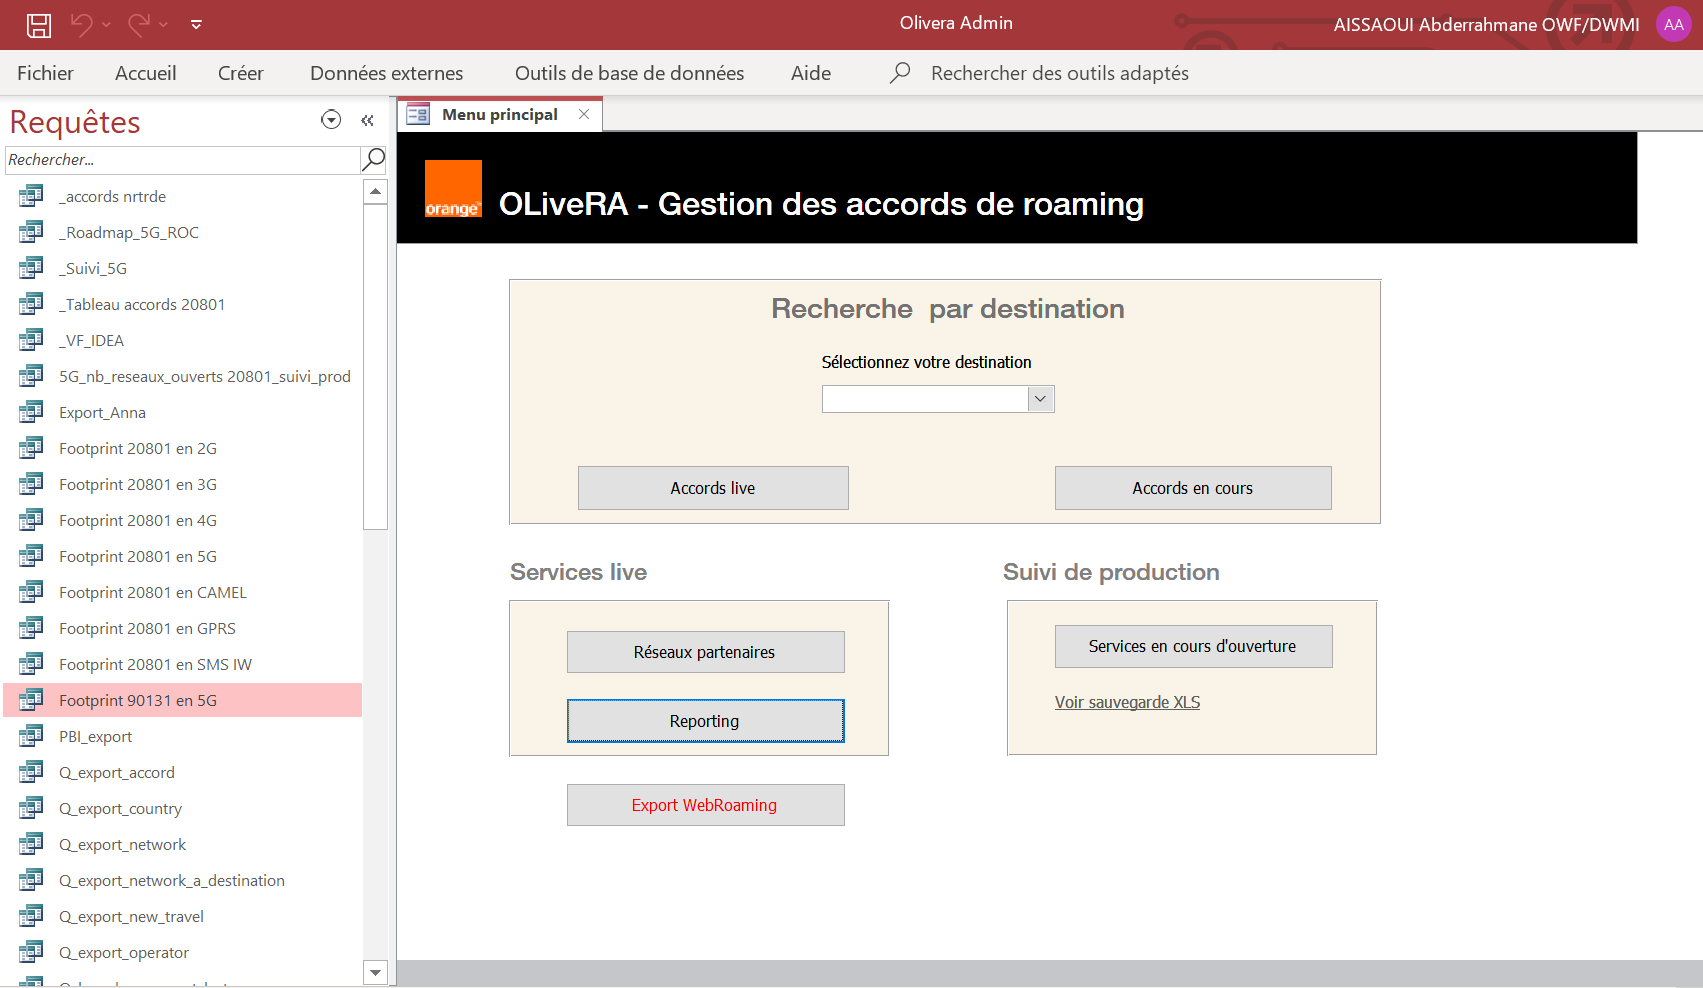
\includegraphics[scale=0.5]{annexs/Olivera 1ST.PNG}
\end{center}

\subsubsection*{Services opening in progress – List of operators in progress}
\begin{center}
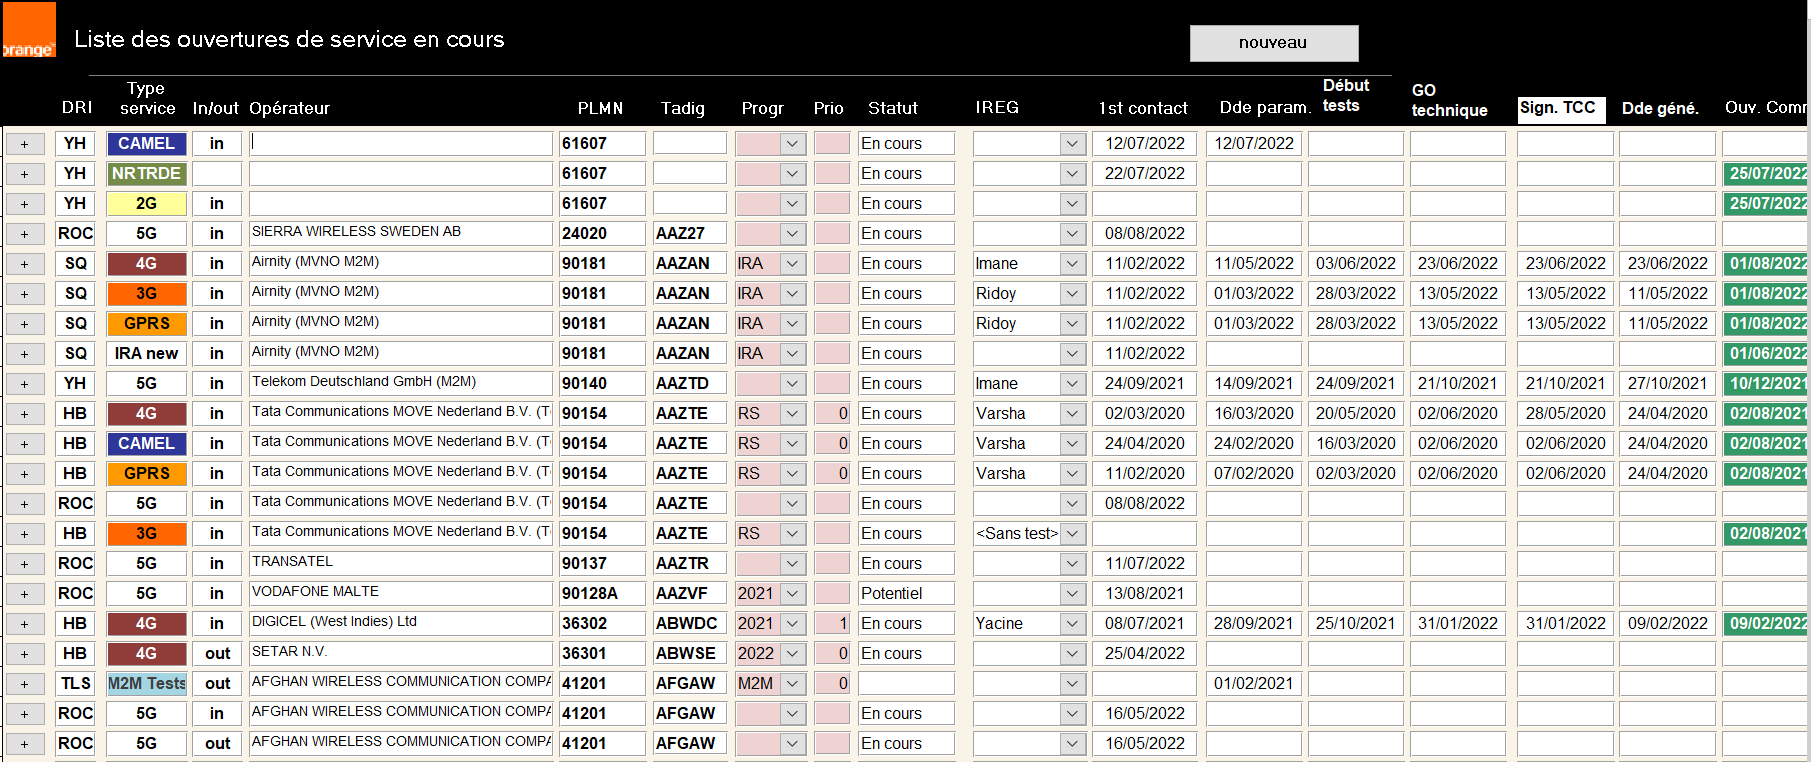
\includegraphics[scale=0.45]{annexs/oliv 3.PNG}
\end{center}

\subsubsection*{Services opening in progress – Operator form}
\begin{center}
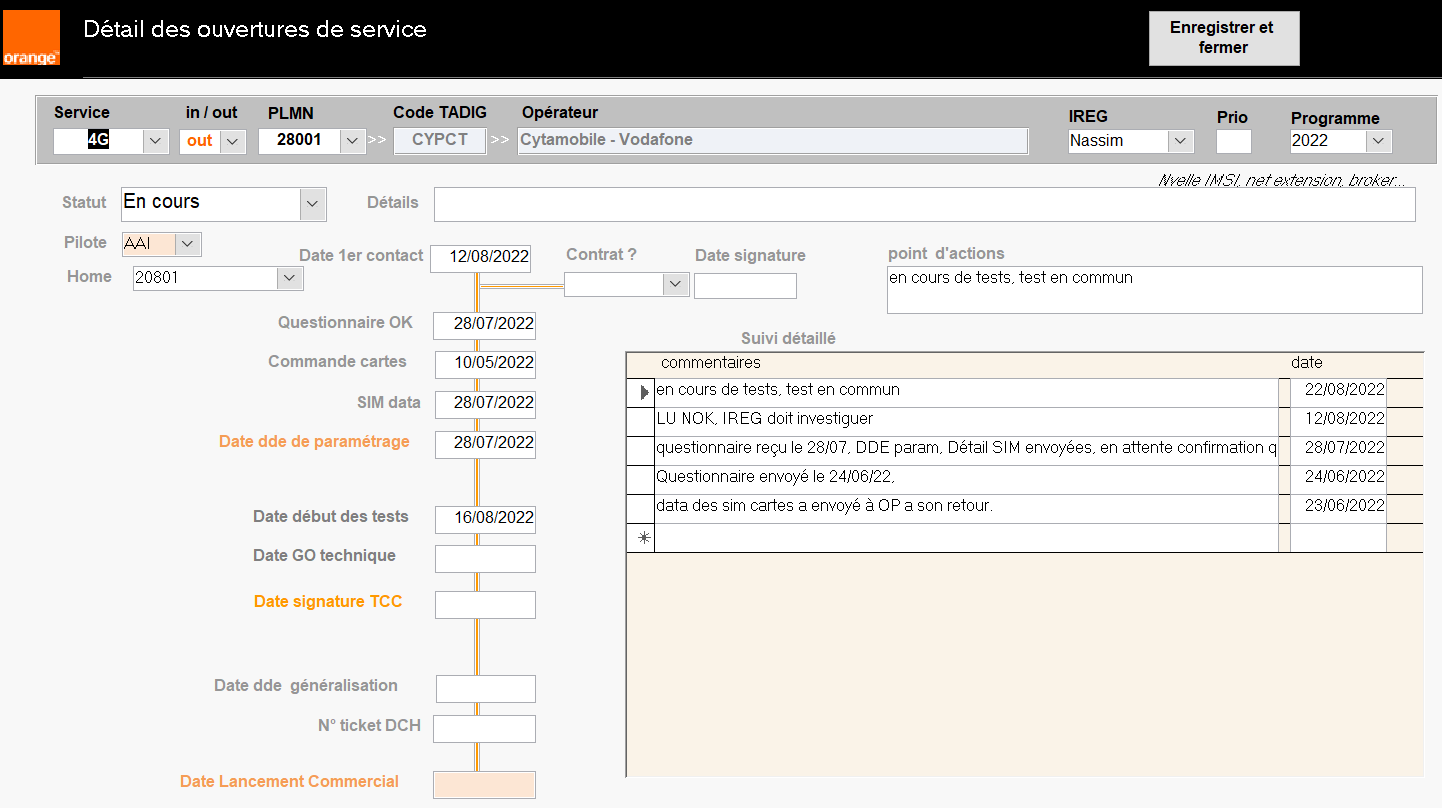
\includegraphics[scale=0.6]{annexs/oliv 4.PNG}
\end{center}

This form contains a certain amount of information necessary for the good follow-up of
the opening process, such as:
\begin{itemize}
    \item The service, as well as a precision on the type of opening (Inbound or Outbound Roaming)
    \item Operator information (PLMN code, TAP code, Commercial name)
    \item All key milestones and it’s dates.
    \item Priority.
    \item Status of contract and tariff negotiations.
    \item The name of the technical expert in charge.
    \item A comment section and an action points section.
\end{itemize}

\subsubsection*{Annex 8 - Overal Roaming Architectur}
\begin{center}
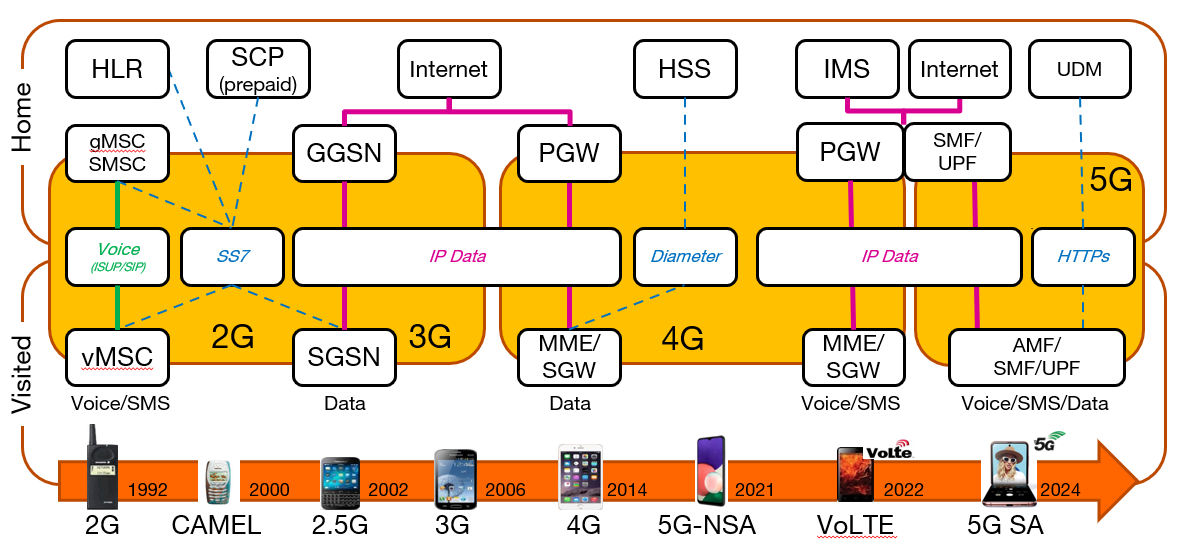
\includegraphics[scale=0.71]{annexs/Overal Roaming services architecture.PNG}
\end{center}

\subsubsection*{Annex 9 - First Page of a \acs{4G} Completed Testbook}
\begin{center}
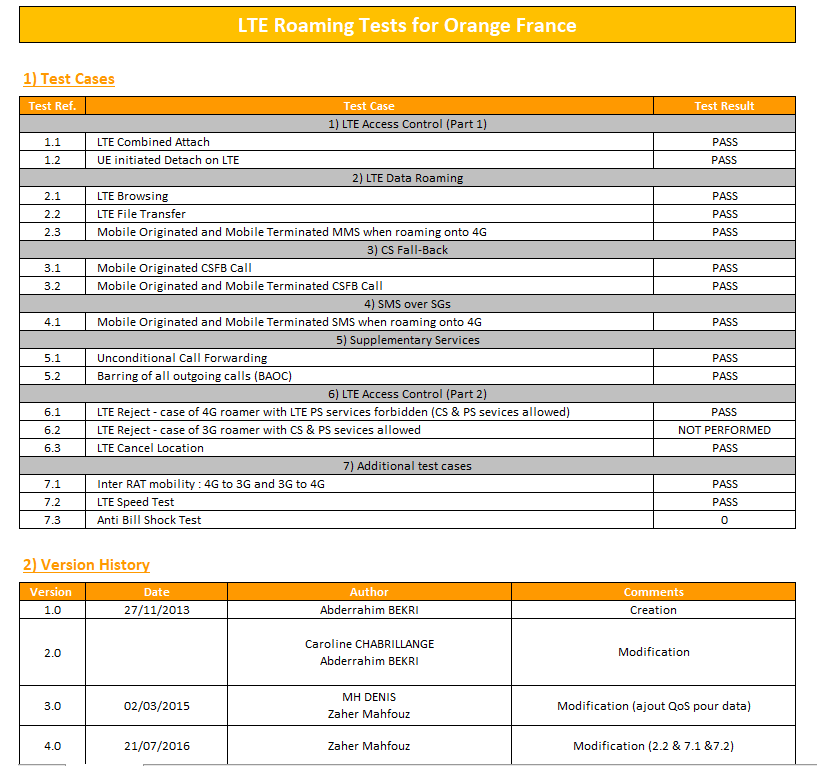
\includegraphics[scale=1]{annexs/LTE roaming test book.PNG}
\end{center}

\subsubsection*{Annex 10 - \acs{SIM} Cards' Data implementation request under VI Networks}
\begin{center}
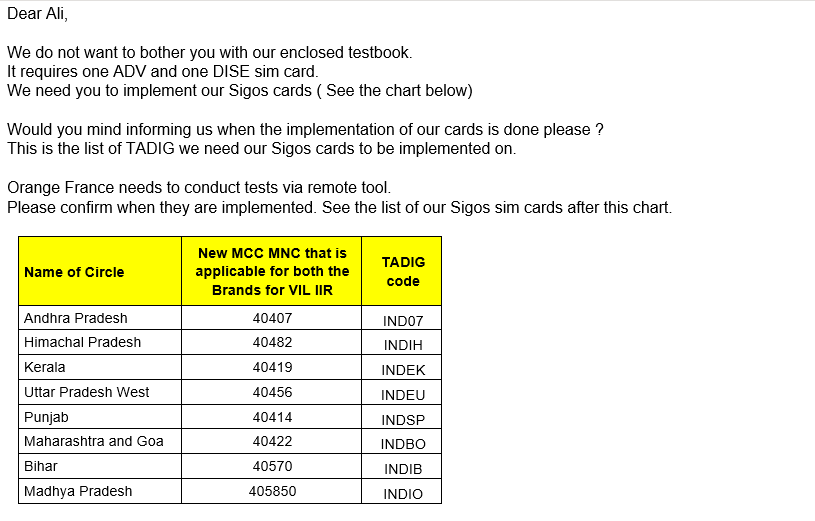
\includegraphics[scale=1.3]{annexs/vimail.PNG}
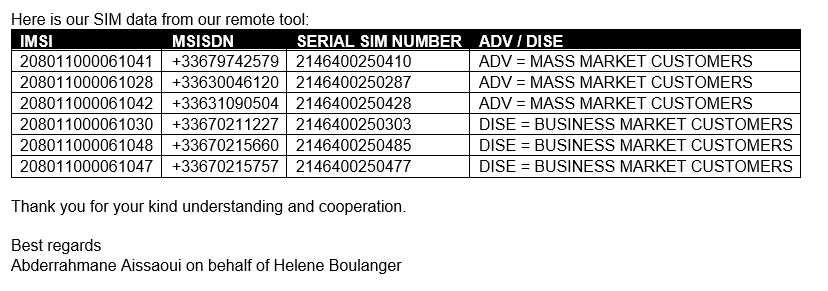
\includegraphics[scale=1.1]{annexs/vimail2.PNG}
\end{center}

\subsubsection*{Annex 11 - CLL Orange Fance - Ooredoo Qatar}
\begin{center}
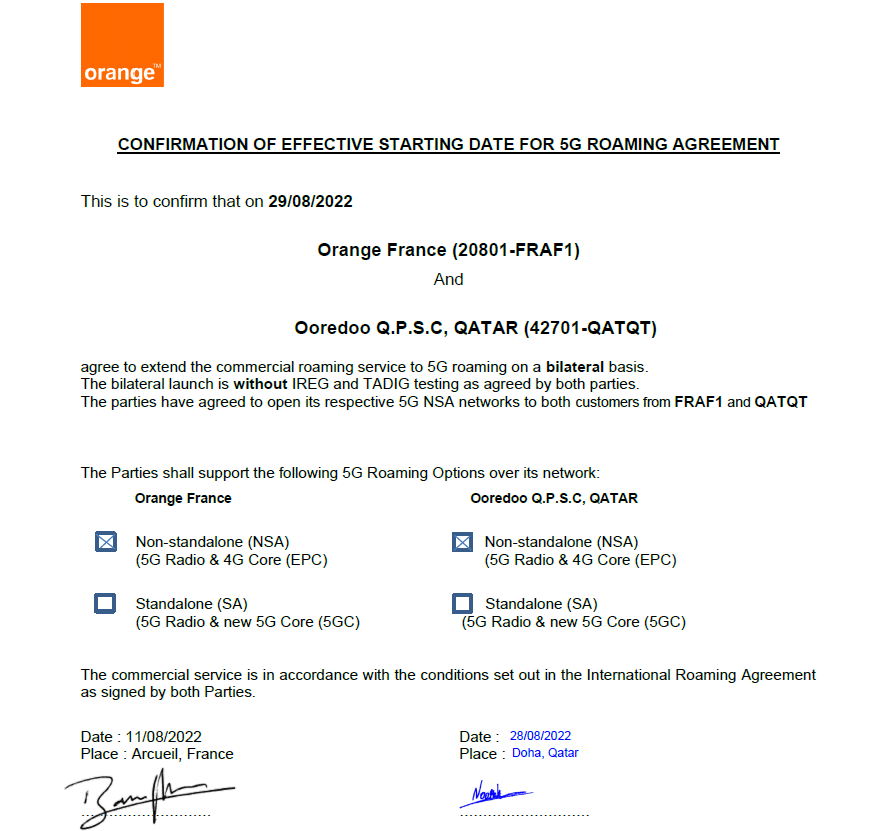
\includegraphics[scale=1.1]{annexs/CLL OOREDOO Quatar.PNG}
\end{center}